\section{Diplomacy}
\subsection{Introduction}
	Diplomacy is currently done by StrategyManager along with other Conditions.
	There are three special conditions created for this purpose:
	\begin{itemize}
		\item ConditionAllied
		\item ConditionNeutral
		\item ConditionHostile
	\end{itemize}
	What they do is check diplomacy against each of the players. Of course it is guaranteed that any two players will be either allies, neutrals or hostiles. Conditions then creates a ``hostile\_player'', ``neutral\_player'' or ''allied\_player'' action that is then passed to BehaviorManager. 
	BehaviorManager asks its BehaviorComponents whether any would be interested in ``solving'' given case. Three special BehaviorComponents are created for this purpose. Each of them is characterized by different traits, so naturally they value different things in other players in game.
	\begin{enumerate}
		\item BehaviorEvil
			\begin{enumerate}
				\item Things it likes in other players: \textbf{strength, large terrain, wealth}.
			\end{enumerate}
		\item BehaviorNeutral
			\begin{enumerate}
				\item Things it likes in other players: \textbf{strength}.
				\item Neutral about \textbf{wealth, terrain size}
			\end{enumerate}
		\item BehaviorGood
			\begin{enumerate}
				\item Things it likes in other players: \textbf{weakness, small terrain}.
				\item Neutral about \textbf{wealth}
			\end{enumerate}
	\end{enumerate}

	Values taken into account are:
	\begin{enumerate}
		\item strength - $( (CHP(ai)) / (CHP(player) ) * ( (lenShips(AI) / (lenShips(player) )$, where CHP(X) is cumulative fighting ship HP of given player X, while lenShips(X) if amount of fighting ships by given player X.
		\item terrain size - $(TSize(ai) / TSize(player)) * (lenIsl(ai) / lenIsl(player))$, where $TSize(X)$ is amount of ground tiles owned by given player, and $lenIsl(X)$ is amount of separate islands owner by given player.
		\item wealth - $(Wres * Res(ai) + Wgold * Gold(ai) / (Wres * Res(player) + Wgold * Gold(player))$ - Where $Res(X)$ is total worth of resources by given player, and $Gold(X)$ is amount of Gold by given player. $Wres$ and $Wgold$ are weights each values has in equation. Currently $Wres = 0.75$ while $Wgold = 0.25$, so resources are valued three times as much as raw gold.
	\end{enumerate}
\subsection{Relationship score}

\begin{par}
	Note that every value \textbf{strength, terrain size} and \textbf{wealth} is not a concrete number, but a balance between AI and other player.
	Theoretically, values of balance are in range of $(0, \infty)$, where values like $0.5$ mean that other player is twice as strong/big/wealthy as AI. 
	Similarly balance value of $3.0$ would mean that AI is three times as strong/big/wealthy as the player it was matched against. 
	To make it simpler, this value is first trimmed to range of 0.1 and 10.0 (to avoid handling zeroes and infinities we assume $balance > 10.0$ is 10.0 and $balance < 0.1$ is 0.1).
	Later, this trimmed value is translated into continuous scale of -10.0 to 10.0, where -10.0 states that given player was close to 10 times weaker than AI (values near 10.0 stating the exact opposite).
\end{par}
\begin{par}
	So what we have so far are three values from a range of $(-10.0, 10.0)$ stating how given player compares to AI.
	As said previously, AI can have any of the three Behaviors defined, that handle diplomacy (\textbf{Evil, Neutral} and \textbf{Good}). To simulate ``preference'' of each behavior, they have weights defined for each of the balance values.
	Evil behavior can have these settings to simulate fondness for strength, large terrains and wealth:
	\begin{itemize}
		\item 'power': -0.6
		\item 'terrain': -0.3
		\item 'wealth': -0.1
	\end{itemize}
	Negative weights mean that in case where enemy is stronger than AI (negative balance), AI takes that as an advantage (higher chance to form an alliance with player)
	Final value is calculated by multiplying weights with corresponding balance values. All weights sum up to values between -1.0 and 1.0 to make sure the final value ($weights * balances$) is between -10.0 and 10.0.
\end{par}

\begin{par}
	What we have right now, is a single real value describing how given Behavior (\textbf{Evil, Neutral} or \textbf{Good}) respects, or ``likes'' given player.
	What we would like right now, is to simulate a scenario where low values ($ < 0.0$) tend to start wars with given AI, while high values ($> 0.0$) make AI form an alliance with given player.
	We could two single threshold values (e.g. $war = -5.0$, $peace = 6.5$) and then have some randomness that decides whether to start a war yet or not. 
	In this case value of -10.0 and -5.0001 would make no difference in behavior, so it's not the best solution.
	Instead we do something else:
	Each of the three diplomatic Behavior has certain parabolic functions attached to it for each of the types of diplomacy settings against player.
	In other words: BehaviorEvil (and the remaining two) has three functions defined for cases where enemy is \textbf{allied, neutral} and \textbf{hostile}.
	That gives us 9 different functions to define totally. Graphical example of that can be see on image \ref{fig:diplomacy1}. Notice that there's no function defined for "NEUTRAL" action. More on that later.
\end{par}

\begin{figure}[h!]
	\centering
	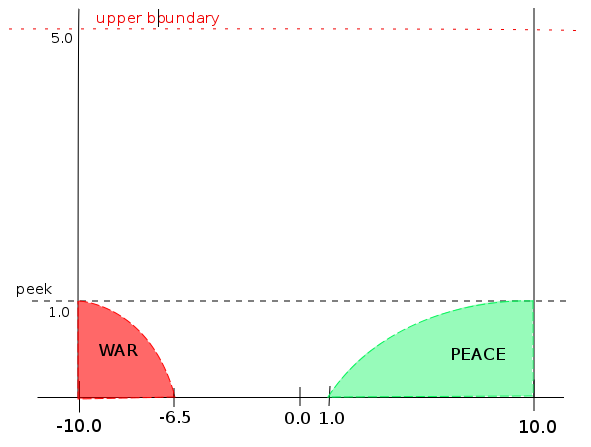
\includegraphics[width=\textwidth]{gfx/diplomacy1.png}
	\caption{Diplomacy settings for ``neutral\_player'' action.}
	\label{fig:diplomacy1}
\end{figure}

\subsection{Example scenario}
\begin{par}
	I know I didn't give out details yet on how the functions work, but let's start out with an example. Let's say $relationship score$ was already calculated against given player (as described earlier) and is equal to \textbf{4.36}.
	Let's also assume it's the case where other player was \textbf{hostile}. See at image \ref{fig:diplomacy2} to have a grasp of how functions could be defined. 
	Notice that player is hostile at that moment, so it should be easy to switch back to peace. 
	We don't have hostility function defined here, because it's the current state of diplomacy between players. 
	"Doing nothing" is also an option when handling diplomacy, so turning hostile again wouldn't really differ from that. 
	Settings show at the figure fit more to Good-natured behavior since it's fairly easy to stop war (all you need is $relationship score$ slightly larger than 0.0.
\end{par}
\begin{par}
	When handling diplomacy, four possible actions can be done:
	\begin{itemize}
		\item WAR - declare war with given player
		\item PEACE - form alliance with given player
		\item NEUTRAL - declare neutrality towards given player
		\item WAIT - do nothing
	\end{itemize}
	Additionally, two random variables may be generated:
	\begin{itemize}
		\item First one states whether any change will be done (see fig. \ref{fig:diplomacy3}) or not. It's equivalent to determining whether random point on a vertical line positioned at $relationship\_value$ would hit yellow or non-yellow pixel. 
		\item If an action was selected (as opposed to waiting), second random variable states which type of action is selected. That's done only when the regions intersect (as shown on fig. \ref{fig:diplomacy3}). Two red spots show probabilities of \textbf{PEACE} and \textbf{NEUTRAL} actions. With $relationship\_value$ fixed at 4.36, \textbf{NEUTRAL} has higher probability to take place.
	\end{itemize}
\end{par}

\subsection{Functions definitions and guidelines on balancing}
	As explained before, we have to define 9 sets of parameters totally. 
	This is done for each of the functions (\textbf{hostile\_player, neutral\_player} and \textbf{allied\_player}) for each of the components (\textbf{BehaviorEvil, BehaviorNeutral} and \textbf{BehaviorGood}), as static parameters in class definition.
	Parameters given for each functions are:
	\begin{itemize}
		\item \textbf{mid} - "Midpoint" or position of the "peek" on X axis (this is fixed for hostile (WAR) and ally (PEACE) functions on -10.0 and 10.0 respectively).
		\item \textbf{root} - point on X axis that's the intersection point of OX axis and function itself. This is somewhat equivalent to $threshold$ value.
		\item \textbf{peek} - how tall should the function be, i.e. what's the maximum value it can achieve at peek point. By default this is 1.0.
	\end{itemize}

	Additionally there's also $upper\_boundary$ value which determines how big the probability to $WAIT$ is.

	Function parameters are provided in each of the BehaviorComponents (Evil, Neutral and Good) in form of a python dictionary, e.g.
\begin{Verbatim}[frame=lines, numbers=left]
	parameters_hostile = {
		'neutral': {'mid': 0.0, 'root': 2.0, 'peek': 0.3, }
		'ally': {'root': 4.0 }
	}
\end{Verbatim}

	To give you a feeling how each parameter alters the chance for given action to be executed, let's use blue function $NEUTRAL$ in \ref{fig:diplomacy2} as an example. 
	High ``peek'' would make the function taller, increasing its chance to be called when the parameter ``relationship\_score'' is somewhere between 0.4 and 6.2). 
	The roots (0.4 and 6.2) would remain the same. If you were to alter the ``root'' parameter, you'd make function broader. 
	Function shown on the figure has parameters 'mid' and 'root' equal to 2.9 and 0.4 respectively (notice that parameters like 2.9 and 6.2 would return the same function). 
	Notice that 'root' parameter is simply a point on OX that the function should intersect, so it's directly connected with it's 'mid' value.
\subsection{Characteristics of the model}
	Model comes with certain advantages and disadvantages.
	\begin{itemize}
		\item Advantages:
			\begin{enumerate}
				\item Relatively few values are needed to define by hand in order to have good results.
				\item upper\_boundary value which allows to ``globally'' make all actions appear less or more often
			\end{enumerate}
		\item Disadvantages:
			\begin{enumerate}
				\item As it comes with heuristic models, it's not perfect.
				\item Quadratic function ($x^{2}$) is used, currently it's not possible to provide other functions, but it's easy to add.
			\end{enumerate}
	\end{itemize}

\begin{figure}[h!]
	\centering
	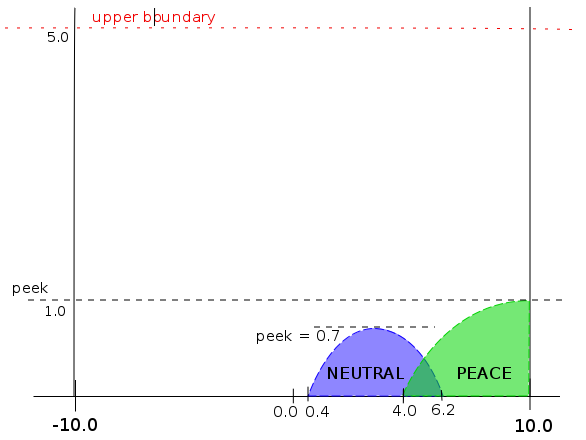
\includegraphics[width=\textwidth]{gfx/diplomacy2.png}
	\caption{Diplomacy for ``hostile\_player'' action.}
	\label{fig:diplomacy2}
\end{figure}

\begin{figure}[h!]
	\centering
	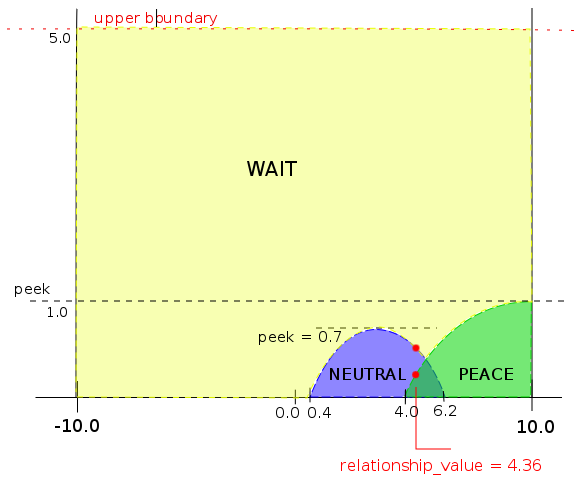
\includegraphics[width=\textwidth]{gfx/diplomacy3.png}
	\caption{Diplomacy for ``hostile\_player'' action.}
	\label{fig:diplomacy3}
\end{figure}
